\chapter{The Main Menu}

\section{Introducing the Main Menu}
\begin{center}
  \includegraphics[width=4cm]{main_menu/images/ss-main-menu-\genericimg.png}
\end{center}
This is the screen from which the rest of the Rockbox functions can be accessed.  It is used for a variety of functions, which are detailed below. All options in Rockbox can be controlled via this menu.

All settings are persistently stored on the unit. However, Rockbox does not spin up the disk solely for the purpose of saving settings, but instead will save them when it spins up the disk the next time, for example when refilling the MP3 buffer or navigating through the file browser. Changes to settings may therefore not be saved unless the \dap is shut down safely (see page \pageref{ref:Safeshutdown}).

The two settings menus are covered in detail starting on page \pageref{ref:configure_rockbox}. All the other options on the main menu are explained here.

Navigating through the menu:

\opt{recorder,recorderv2fm,ondio,h1xx,h300,ipodnano,ipodcolor,ipodvideo}{
\begin{table}[h!]
    \begin{center}
      \begin{tabular}{@{}lc@{}}\toprule
       \textbf{Key} & \textbf{Action} \\\midrule
        UP & Moves up in the menu. \\
           & Inside a setting, increases the value or chooses next option \\
        DOWN & Moves down in the menu. \\
             & Inside a setting, decreases the value or chooses previous option \\
        PLAY/RIGHT & Selects option \\
        OFF/LEFT & Exits menu, setting or moves to parent menu\\\bottomrule
      \end{tabular}
    \end{center}
\end{table}
}
\opt{player}{
\begin{table}[h!]
  \begin{center}
    \begin{tabular}{@{}cc@{}}\toprule
      \textbf{Key} & \textbf{Action} \\\midrule
      MINUS & Selects previous option in the menu. \\
            & Inside an setting, decreases the value or chooses previous option \\
      PLUS & Selects next option in the menu. \\
           & Inside an setting increases the value or chooses next option \\
      PLAY & Selects item \\
      STOP & Exit menu, setting or moves to parent menu. \\\bottomrule
    \end{tabular}
  \end{center}
\end{table}
}

\section{\label{ref:Recording}Recording}
\subsection{\label{ref:Whilerecordingscreen}While Recording Screen}
\begin{center}
  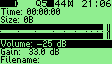
\includegraphics[width=4cm]{main_menu/images/ss-while-recording-screen-112x64x1.png}
\end{center}

Entering the ``Recording'' option in the Main menu launches the recording application. The screen shows the time elapsed and the size of the file being recorded. A peak meter is present to allow you set Gain correctly.  The frequency, channels and quality settings are shown on the last line.

The controls for this screen are:

\begin{table}[h!]
  \begin{center}
    \begin{tabular}{@{}cc@{}}\toprule
      \textbf{Button} & \textbf{Function} \\\midrule
      LEFT & Decreases Gain \\
      RIGHT & Increases Gain \\
      PLAY & Starts recording.  \\
           & While recording, button closes the current file and opens a new one.\\
           & (while recording) Pauses / restarts recording \\
      STOP & Exits Recording Screen.\\
           & (while recording) Stop recording \\
      F1 & Opens Recording Settings screen (see below) \\
      F2 & Quick menu for recording settings. \\
         & A quick press will leave the screen up (press F2 again to exit),\\
         & while holding it will close the screen when you release it. \\
      F3 & Quick menu for source setting. \\
         & Quick/hold works as for F2. \\
         & (while recording) Start a new recording file \\\bottomrule
    \end{tabular}
  \end{center}
\end{table}

\subsubsection{\label{ref:Recordingsettings}Recording Settings}
\begin{itemize}
\item \textbf{Quality}
  Choose the quality here (0 to 7). Default is 5, best quality is 7, smallest file size is 0.  This setting effects how much your sound sample will be compressed.  Higher quality settings result in larger MP3 files.

  The quality setting is just a way of selecting an average bit rate, or number of  bits per second, for a recording.  When  this setting is lowered, recordings are compressed more (meaning worse sound quality), and the average bitrate changes as follows.
\end{itemize}

\begin{table}[h!]
  \begin{center}
    \begin{tabular}{@{}ll@{}}\toprule
      \textbf{Frequency} & \textbf{Bitrate}  (Kbit/s) {}- quality 0{}-{\textgreater}7 \\\midrule
      44100Hz stereo: & 75, 80, 90, 100, 120, 140, 160, 170 \\
      22050Hz stereo & 39, 41, 45, 50, 60, 80, 110, 130 \\
      44100Hz mono & 65, 68, 73, 80, 90, 105, 125, 140 \\
      22050Hz mono & 35, 38, 40, 45, 50, 60, 75, 90 \\\bottomrule
    \end{tabular}
  \end{center}
\end{table}

\begin{itemize}
\item \textbf{Frequency} 
Choose the recording frequency (sample rate) {}- 48kHz, 44.1kHz, 32kHz (MPEG version 1), and 24kHz, 22.05kHz, 16kHz (MPEG version 2) are available.  Higher sample rates use up more disk space, but give better sound quality.  This setting determines which frequency range can accurately be reproduced during playback. Lower frequencies produce smaller files, for two reasons.  The amount of data to be compressed is smaller and the data is easier to compress, since higher frequencies are not present.  The frequency setting also determines which version of the MPEG standard sound is recorded using.

\item \textbf{Source}
Choose the source of the recording.  This can be microphone, line in, or SPDIF (digital). For recording from the radio on the FM recorder, see page \pageref{ref:FMradio}.

Note: you cannot change the sample rate for digital recordings.

\item \textbf{Channels}
This allows you to select mono or stereo recording.  Please note that for mono recording, only the left channel is recorded.  Mono recordings are usually somewhat smaller than stereo.

\item \textbf{Independent Frames}
The independent frames option tells the \dap to encode with the bit reservoir disabled, so the frames are independent of each other. This makes a file easier to edit.

\item \textbf{Time Split}
This option is useful when timing recordings. If set to active it stops a recording at a given interval and then starts recording again with a new file., which is useful for long term recordings.

The splits are seamless (frame accurate), no audio is lost at the split point. The break between recordings is only the time required to stop and restart the recording, on the order of 2{}-4 seconds.

Options (hours:minutes between splits): off, 24:00, 18:00, 12:00, 10:00, 8:00, 6:00, 4:00, 2:00, 1:20 (80 minute CD), 1:14 (74 minute  CD), 1:00, 00:30, 00:15, 00:10, 00:05.
\item \textbf{Prerecord Time}
This setting buffers a small amount of audio so that when the record button is pressed, the recording will begin from that number of seconds earlier.  This is useful for ensuring that a recording begins before a cue that is being waited for.\\
Options: Off, 1{}-30 seconds
\end{itemize}

\section{\label{ref:FMradio}FM Radio}
\begin{center}
  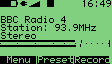
\includegraphics[width=4cm]{main_menu/images/ss-fm-radio-screen-112x64x1.png}
\end{center}
This menu option switches to the radio screen. 

The keys are:

\begin{table}[h!]
  \begin{center}
    \begin{tabular}{@{}lc@{}}\toprule
      \textbf{Button} & \textbf{Function} \\\midrule
      LEFT, RIGHT & Change frequency in 0.1 MHz steps. \\
                  & For automatic station seek, \\
                  & hold LEFT/RIGHT for a little longer. \\
      UP, DOWN & Change volume \\
      PLAY & \textbf{(EXPERIMENTAL)} freezes all screen updates.\\
           & May enhance radio reception in some cases. \\
      ON & Leave the radio screen with the radio playing \\
      OFF & Back to main menu \\\bottomrule
    \end{tabular}
  \end{center}
\end{table}
The FM radio has the ability to record and to remember station frequency settings (presets).

\begin{itemize}

\item \textbf{Saving a preset}
You can save your favourite stations in the 32 presets. Press F1 to go to the menu, then select ``Save preset''. Enter the name (maximum number of characters is 32).

\item \textbf{Selecting a preset}
Press F2 to go to the preset list. Use UP and DOWN to move the cursor and then press PLAY to select. Use LEFT to leave the preset without selecting anything.

\item \textbf{Removing a preset}
Press F1 to go to the menu, then select ``Remove preset''.

\item \textbf{Recording}
Press F3 to start recording the currently playing station. Press OFF to stop recording. Press PLAY again to seamlessly start recording to a new file. The settings for the recording can be changed in the F1 menu before starting the recording. See page \pageref{ref:Recordingsettings} for details of recording settings.

Note: The radio will turn off when playing an MP3.
\end{itemize}

\section{\label{ref:Bookmarkconfig}\label{ref:Bookmarkmenu}Bookmarks}
The bookmarks menu allows you to create and manage bookmark files.

\begin{itemize}

\item \textbf{Create Bookmark}
While playing a track, use this option to save your current position within the track so that you can return to it at a later time.  Bookmarks are saved on a per folder basis i.e. all of the files in the same folder have their bookmarks stored together. You can store multiple bookmarks for the same track.

\item \textbf{List Bookmarks}
\begin{center}
  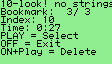
\includegraphics[width=4cm]{main_menu/images/ss-list-bookmarks-112x64x1.png}
\end{center}
%\includegraphics[width=4.669cm,height=2.006cm]{images/rockbox-manual-img31.png} 
While playing a track, use this option to return to any bookmark in the current folder.  The bookmark browser screen (shown above) is now displayed.  Use the UP and DOWN keys (recorder) or MINUS and PLUS keys (player) to navigate between bookmarks.  Press PLAY to jump to a bookmark, ON+PLAY to delete a bookmark or STOP/OFF to exit the browser.

\item \textbf {Recent bookmarks}
If the ``save a list of recently created bookmarks'' option is enabled then you can view a list of several recent bookmarks here and select one to jump straight to that track.  This option is off by default. See page \pageref{ref:Bookmarkconfigactual} for more details on configuring bookmarking in Rockbox.
\end{itemize}

\section{\label{ref:playlistoptions}Playlist Options}
This menu allows you to work with playlists. Playlists can either be created automatically by playing a file in a directory directly, which will cause all of the files in that directory to be placed in the playlist, or they can be created by hand using the File Menu (see page \pageref{ref:Filemenu}) or using the Playlist Options menu.  Both  automatic and manually created playlists can be edited using this menu.

\begin{itemize}
\item \textbf{Create Playlist}
Rockbox will create a playlist with all tracks in the current directory and all subdirectories. The playlist will be created one folder level ``up'' from
where you currently are. 

\item \textbf{View Current Playlist}
Displays the contents of the playlist currently stored in memory.

\item \textbf{Save Current Playlist}
Saves the current dynamic playlist, excluding queued tracks, to the specified file. If no path is provided then playlist is saved to current directory (see page \pageref{ref:Playlistsubmenu}).

\item \textbf{Recursively Insert Directories}
If set to ON then when you insert/queue a directory in Dynamic Playlist, all subdirectories will also be inserted. If set to ASK then you are prompted about recursive insertion when inserting a directory.
\end{itemize}

\section{Browse Plugins}
With this option you can load and run various plugins that have been written for Rockbox.\\

A detailed description of the different plugins begins on page \pageref{ref:Part5}.

\section{\label{ref:Info}Info}
This option shows MP3 ram buffer size, battery voltage level and estimated time remaining, disk total space and disk free space.
On players use the MINUS and PLUS keys to step through several pages of information.

\begin{itemize}

\item \textbf{Show ID3 info}
This is an alternative way to access the ID3 viewer.  See page \pageref{ref:ID3viewer} for details on the ID3 viewer.
\item \textbf{Rockbox Info}
Displays some basic system information.  This is, from top to bottom, the amount of memory Rockbox has available for storing music (the buffer), battery status, hard disk size and the amount of free space on the disk.

\item \textbf{Version}
Software version and credits display.

\item \textbf{Debug (Keep Out!)}
This submenu is intended to be used only by Rockbox developers. It shows hardware, disk, battery status and a lot of other information.  It is not recommended that users access this menu unless instructed to do so in the course of fixing a problem with Rockbox.  In particular the ``Dump ROM Contents'', ``View/clear RTC RAM'' and ``Screenshot'' and ``Sound test'' functions should be treated with care.
\end{itemize}

\section{Shutdown (Player)}
This menu option saves the Rockbox configuration and turns off the hard drive before shutting down the machine. For maximum safety this procedure is recommended when turning off the Jukebox. (There is a very small risk of hard disk corruption otherwise.) See page \pageref{ref:Safeshutdown} for more details.
